\documentclass{article}
\usepackage[margin=.5in]{geometry}
\usepackage{graphicx, dblfloatfix}
\usepackage{amsmath, amssymb, amsfonts, mathrsfs, mathtools}
\usepackage[english]{babel}
\usepackage[autostyle, english = american]{csquotes}
\usepackage[normalem]{ulem}
\usepackage[title,titletoc,toc]{appendix}
\usepackage{pgfplotstable}
\usepackage{array, booktabs, colortbl}
\MakeOuterQuote{"}

\pgfplotsset{compat=1.12}


\newcommand{\redchi}{$\tilde{\chi}^2\,$}
\DeclareMathOperator{\erf}{erf}
\DeclareMathOperator{\cov}{cov}
\DeclarePairedDelimiter\abs{\lvert}{\rvert}%
\DeclarePairedDelimiter{\parens}{\lparen}{\rparen}

\title{Single Photon Interference}
\author{Aman LaChapelle}

\begin{document}
\raggedright
\maketitle

\begin{abstract}
	We present here a method by which we can determine the wave-particle duality of light and show that it is a quantum-mechanical and that they comprise parts of a system that is not possible to describe classically.  In all, we are able to show several effects, each can be described classically on its own, but the combination of all these effects can only be described using quantum mechanics.
\end{abstract}

\tableofcontents
\newpage

\section{Introduction}
	It is generally well known that light has both particle-like qualities, in that it carries momentum, and that it can act like a quantum mechanical particle system in that its motion and other properties can be described in real space as well as in momentum space (roughly) with the free particle hamiltonian, especially in the regime where we have not engineered photon-photon interactions.  In general, we can use a faily standard probablistic interpretation in order to understand the way that light behaves given different situations.  In our particular case, we can understand the physical differences between distinguishable paths, indistinguishable paths, and ***erasure of interference that we can directly cause with a polarizing filter.


\section{Theory}
	An important property of interfering a photon with itself is that if we perform the experiment in such a way that the paths of the photon \emph{could} be distinguished, we do not in fact actually have to realize measurement of the difference between the paths of the photon.  In essence, what we can and will do is impose a polarization condition on the two arms of the interferometer.

	\subsection{Classical Photons}
	What we have discussed so far is, however, a quantum mechanical observation.  We can describe each of these situations classically by considering the polarization and co-propagation of the EM waves that make up the laser beam.  We will consider each of the three cases separately and begin to explore the classical electrodynamic explanation for these three phenomena.

	\hspace{.5cm}

	The first case we will consider is the case where the two paths the photon could take are indistinguishable.  Take the polarization of the photon(s) to be uniform across the two paths, and take the $\hat{z}$ to be the direction of propagation of the waves, so our wave vector $\vec{k} = \abs{k}\hat{z}$.  If we make the reasonable assumption that these photons propagate in what is approximately free space, we can write down the $\vec{E}$ and $\vec{B}$ fields like so:

	\begin{gather}
		\vec{E} \, \text{or} \, \vec{B} = Ae^{i(\vec{k} \cdot \vec{r} - \omega t)} + Be^{-i(\vec{k} \cdot \vec{r} - \omega t)}\\
		\vec{E} = \parens*{Ae^{i(kz-\omega t)} + Be^{-i(kz-\omega t)}}\hat{x}\\
		\vec{B} = \parens*{Ae^{i(kz-\omega t)} + Be^{-i(kz-\omega t)}}\hat{y}
	\end{gather}

	where we have arbitrarily chosen that the photon (by convention, $\vec{E}$) is polarized in $\hat{x}$.  Because we can simply choose our axes such that this occurs, we would be able to arbitrarily realign such that this is the case, or any of the orthogonal directions points along the polarization direction.  The most important thing to note here is that the $\vec{E}$, $\vec{B}$, and $\vec{k}$ are all orthogonal.  $A$ and $B$ are arbirtary scale constants.  There are relations between the $\vec{E}$ and $\vec{B}$ fields that we simply absorb into these constants.

	\hspace{.5cm}

	Classically, when we send a wave through a beam splitter, like the EM waves that make up photons, we expect that the wave will split as it passes through one arm of the interferometer, and that when the waves recombine we will see a phase difference that causes an interference effect as long as the path lengths are different.  When the waves recombine, they simply superimpose upon one another.  If the phases of those waves is different when they recombine, we will see an interference pattern - in some places they will interfere constructively and in others destructively as we would expect from any other wave.

	\hspace{.5cm}

	Now we consider the case where the two paths are distinguishable - where we have, for example, selected different polarizations for the two waves.  Looking again at equations 2 and 3, we see that the waves should not interfere at all.  If we align the $\vec{E}$ of one arm with the $\vec{B}$ of the other arm, since the waves still propagate in the same direction, we will notice that $\vec{E}$ and $\vec{B}$ of the two arms are orthogonal and as such will not interfere.  If there is still some component of the fields in a parallel direction there will be a small amount of interference, but overall this interference will be very small.  Certainly much smaller than it would be if the waves were aligned.

	\hspace{.5cm}

	Finally, we can consider the case where one wave is polarized just before it hits the APD, but after the two waves through the second beam splitter and recombine in the interferometer.  It is useful to use the following image to imagine not only the first two situations (indistinguishable, distinguishable paths) as well as the one we consider now.

	\begin{figure}[!htb]
		\centering
		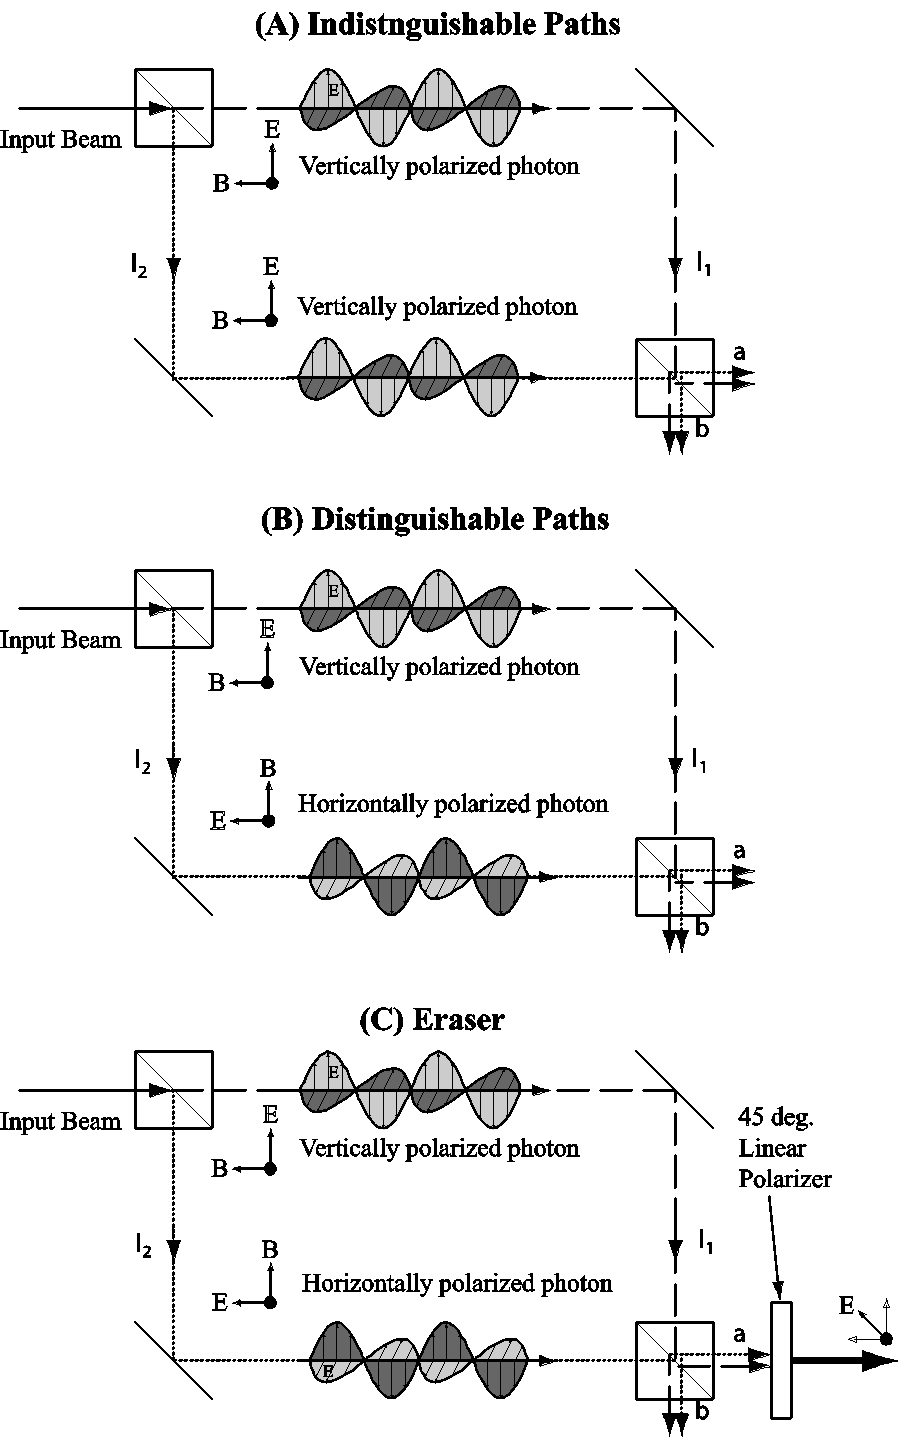
\includegraphics[scale=.5]{interferometer_wave.png}
		\caption{A very classical depiction of a photon interference experiment.  This shows roughly how the waves are passing through the arms of the interferometer.}
	\end{figure}

	In essence, when the waves pass through the second beam splitter, they will recombine, and even though they have opposite polarizations they will still have some phase difference.  When we then pass the waves through the linear polarizer, that phase difference becomes important as the waves are polarized to one direction and the interference pattern is restored.  We would expect to see an interference pattern in the APD that has the linear polarizer in front of it, albeit at a reduced amplitude.  We would expect no interference still at the other APD.

	\subsection{Quantum Photons}
	Quantum particles are fundamentally different from Classical particles.  The primary difference lies in the way that we characterize their position, momentum, and really any quantity about them.  We make use of a probability distribution instead of any certainty in its position/momentum.  In general, we can write the probability as

	\begin{equation*}
		P(\bar{x}) = \abs{\psi(x)}^2.
	\end{equation*}

	If we consider two paths through the interferometer (now jumping to specifics on our experiment), we can write that, assuming the particles (paths) are indistinguishable, $\psi = \psi_1 + \psi_2$.  This results in a probability distribution given by

	\begin{equation}
		P = \abs{\psi_1+\psi_2}^2.
	\end{equation}

	If we now consider that a photon has certain transmission and reflection amplitudes, $t$ and $r$, and plugging into equation 4, 

	\begin{gather}
		P = \abs{tre^{il_1} + tre^{il_2}} \\
		P = rr^* tt^* \parens*{2+tre^{il_1} + tre^{il_2}} \\
		P = 2RT\parens*{1+\cos{\delta}}
	\end{gather}

	where $R$ is the reflection probability, $T$ is the transmission probability and $\delta$ is the phase difference acquired from the difference in the paths.

	If the paths are distinguishable, we add the probability distributions instead of the $\psi$ and so equation 7 becomes

	\begin{gather}
		P = \abs{tre^{il_1}} + \abs{tre^{il_2}} \\
		P = 2RT
	\end{gather}

	If we consider the case of the eraser, where after the polarizing filter the paths are again indistinguishable, we should see again a probability amplitude that depends on the phase difference.  Because this calculation/derivation is long and arduous, we restrict ourselves to quoting the result, 

	\begin{equation}
		P = \frac{1}{4}\parens*{1-\cos{\delta}}.
	\end{equation}

	This is as we would expect, the interference pattern returns, at a diminished amplitude due to the polarizer filtering out some of the photons.

	\hspace{.5cm}

	Now we will examine why we can think about light in terms of quantized packets, rather than as the classical continuum.  Because the BBO crystal emits photons by spontaneous parametric down conversion, we have very simple evidence that the photons are discrete quanta.  Because this only occurs for a very small number of entering photons, i.e. the efficiency is low, we realize that this would not occur for a classical continuous wave.  A continuous wave would be able to split in the same way that the pump photons down-convert, but it would not have a low efficiency - we would still see constant coincidence counts, with each at a reduced amplitude rather than discrete counts (what we observe).

	\hspace{.5cm}

	We can show more rigourously that there is statistically only a single photon passing through the interferometer at a time, i.e. we can show that a photon is a particle by calculating its size in physical space.  We know from the uncertainty principle that

	\begin{equation*}
		\Delta E \Delta t \geq \hbar/2.
	\end{equation*}

	We decompose $\Delta E$ into measureable quantities, like so.

	\begin{gather*}
		\Delta E = \frac{E}{\lambda} \Delta \lambda \\
		\Delta E = \frac{\hbar c}{\lambda^2}\Delta \lambda
	\end{gather*}

	And so now we will be able to find the approximate size in real space of the photon as follows,

	\begin{gather*}
		\Delta t \geq \frac{\hbar}{2\Delta E} \\
		\Delta x \approx c\Delta t \\
		\Delta x \geq c\frac{\hbar}{2\Delta E} = c\frac{\hbar}{2}\frac{\lambda^2}{\hbar c \Delta \lambda} \\
		\Delta x \geq \frac{\lambda^2}{2\Delta \lambda}
	\end{gather*}

	We take the uncertainty in the time to be the uncertainty in when the photon struck the APD.  This means that we don't know exactly when the photon struck, but we can tell that there was a pulse.  Thus we know how long it took the photon to fully strike the APD, and so we know, given the speed of light, how long the photon is.  Since the APD is a physical piece of equipment, it will have a certain resolution.  That will give us the uncertainty in $\lambda$, allowing us to calculate the length of the photon.  Given this value, we are then able to calculate (given singles counts of the APD and the time between counts) the average distance between the photons.  This will let us show that it is incredibly unlikely that any more than one single photon passes through the interferometer at any given time.  We will perform the actual calculation later on, but we establish the theory behind the calculation here.

	\hspace{.5cm}

	There is a significant problem with this theory that we have laid down, and that is that we haven't truly established whether photons are particles.  All of the features of photons that we have observed could be explained by a wave packet.  It is possible to have a wave packet that is localized in space, and have it also split at the beam splitter.  We can, however, show that photons have both natures, both wave and particle.

	\hspace{.5cm}

	Consider, for example, an experiment in which we insert a beam splitter between two APDs.  Then, we consider the coincidence rates between the two APDs.  If this was a wave packet, we would expect to see some nontrivial coincidence rates even when the laser is on.  Since a wave packet can be split like any other wave, it is not unreasonable to expect that each such wave packet will do so and produce a coincidence countrate that is far above the accidental rates.  We will find, however, that this is not the case.  Because the photons are both waves and particles, we will find that they share some of the indivisibiity properties of particles.  Given this information, we will realize that we cannot reconcile the classical arguments for the nature of a photon given the fact that if only one photon passes through the interferometer, and the fact that it does not split.  In fact, we realize that the only possible manner of interaction is for the photon to interfere with itself, in that it has a finite probability of traveling down both arms of the interferometer at once.

	\hspace{.5cm}

	In the interest of completeness, we should mention that light travels extremely fast.  As a consequence of this, since the APD has only about a 58\% efficiency \cite{eff} - meaning that only about half the photons incident on the lens actually cause a count to occur.  Thus it is possible that a photon could bounce off the lens and into the other APD, while the next photon behind it causes a count in the first APD, causing an accidental coincidence.  This is not terribly unlikely, and in fact it probably does happen.  However, the geometry of the APDs is such that it happens extremely rarely, and is thus on a level that is comparable to the background that we would expect, and account for.

\section{Apparatus}

\begin{figure}[!htb]
	\centering
	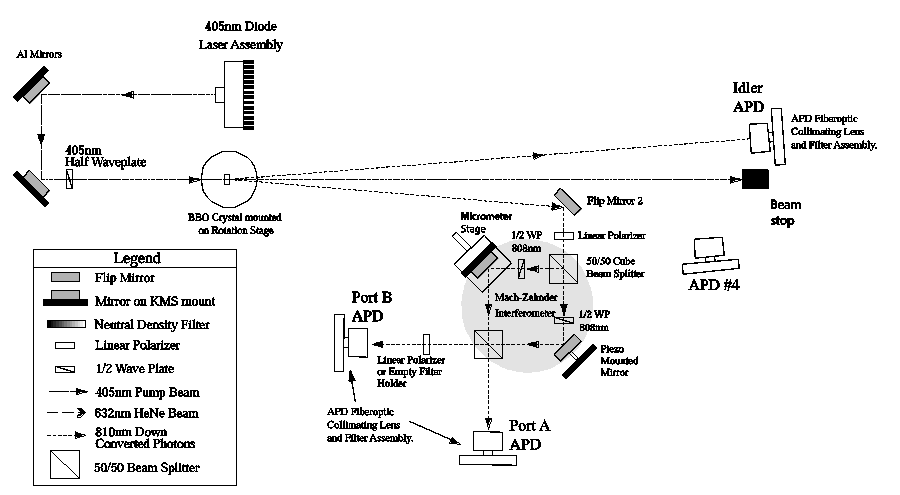
\includegraphics[scale=.5]{apparatus_setup.png}
	\caption{A schematic of the optical table as seen from above.  The APD letters correspond to numbers.  We attempt to keep the naming convention that uses the numerical representation, however.}
\end{figure}

An optical table is an extremely sensitive experimental setup.  We were fortunate that the alignment for the optical table was done for us, the only task that remained was for us to place and align a beam splitter between APD 1 and 4 (Idler and \#4), and to place a linear polarizer between APD 2 (Port B) and the recombining beam splitter of the Mach-Zhender interferometer.

\hspace{.5cm}

Much of the information on the interferometer and the optical setup is superfluous and so I will refrain from mentioning it here.  However, it is important to note that one of the mirrors is mounted on a piezo crystal that allows us to control the path length by varying the voltage applied to the crystal.  This causes the crystal to grow predictably, and allows us to vary path length by an amount that is well known.  Figure 3 is included for clarity and to show which arm of the interferometer has its length adjusted.

\begin{figure}[!htb]
	\centering
	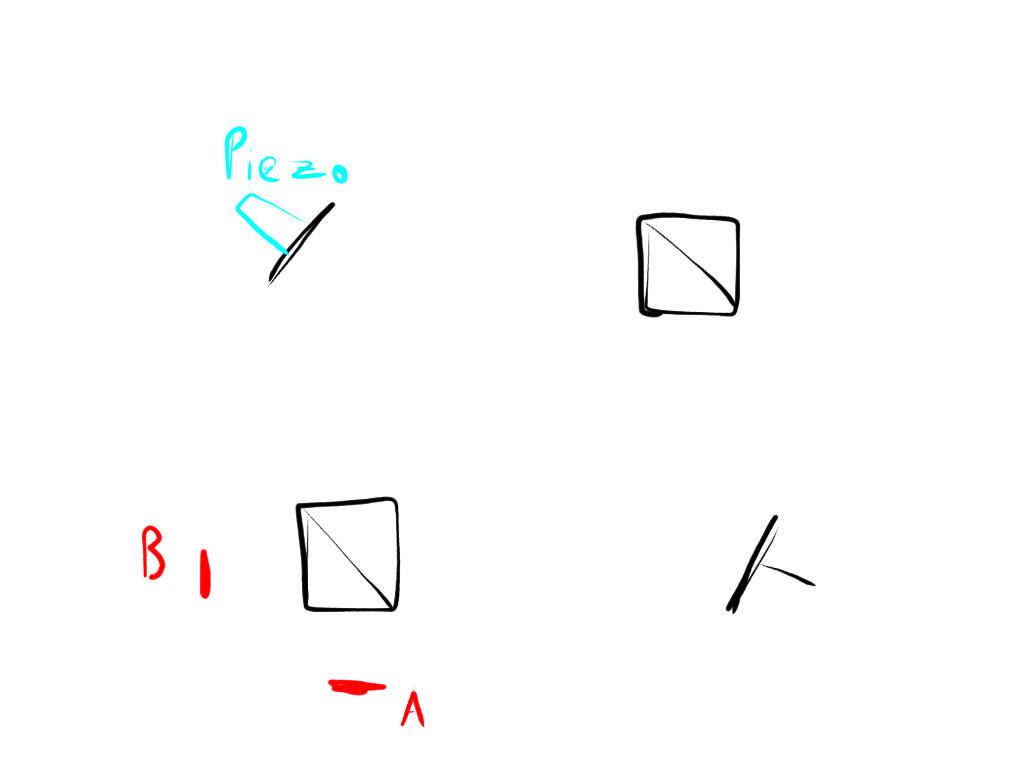
\includegraphics[scale=.3]{interferometer_sketch.jpg}
	\caption{A rough rendering of the interferometer detail.}
\end{figure}



\section{Data/Uncertainty Analysis}

We will begin with the case where the paths of the photon are indistinguishable and show the interference pattern.  Then we will move on to the case where the paths are, in principle distinguishable, and finally we will show the case where the paths are distinguishable before the photons hit the second linear polarizer and afterwards the paths are again indistinguishable, resulting in a return of the interference pattern but only in one APD.

\begin{figure}[!htb]
	\centering
	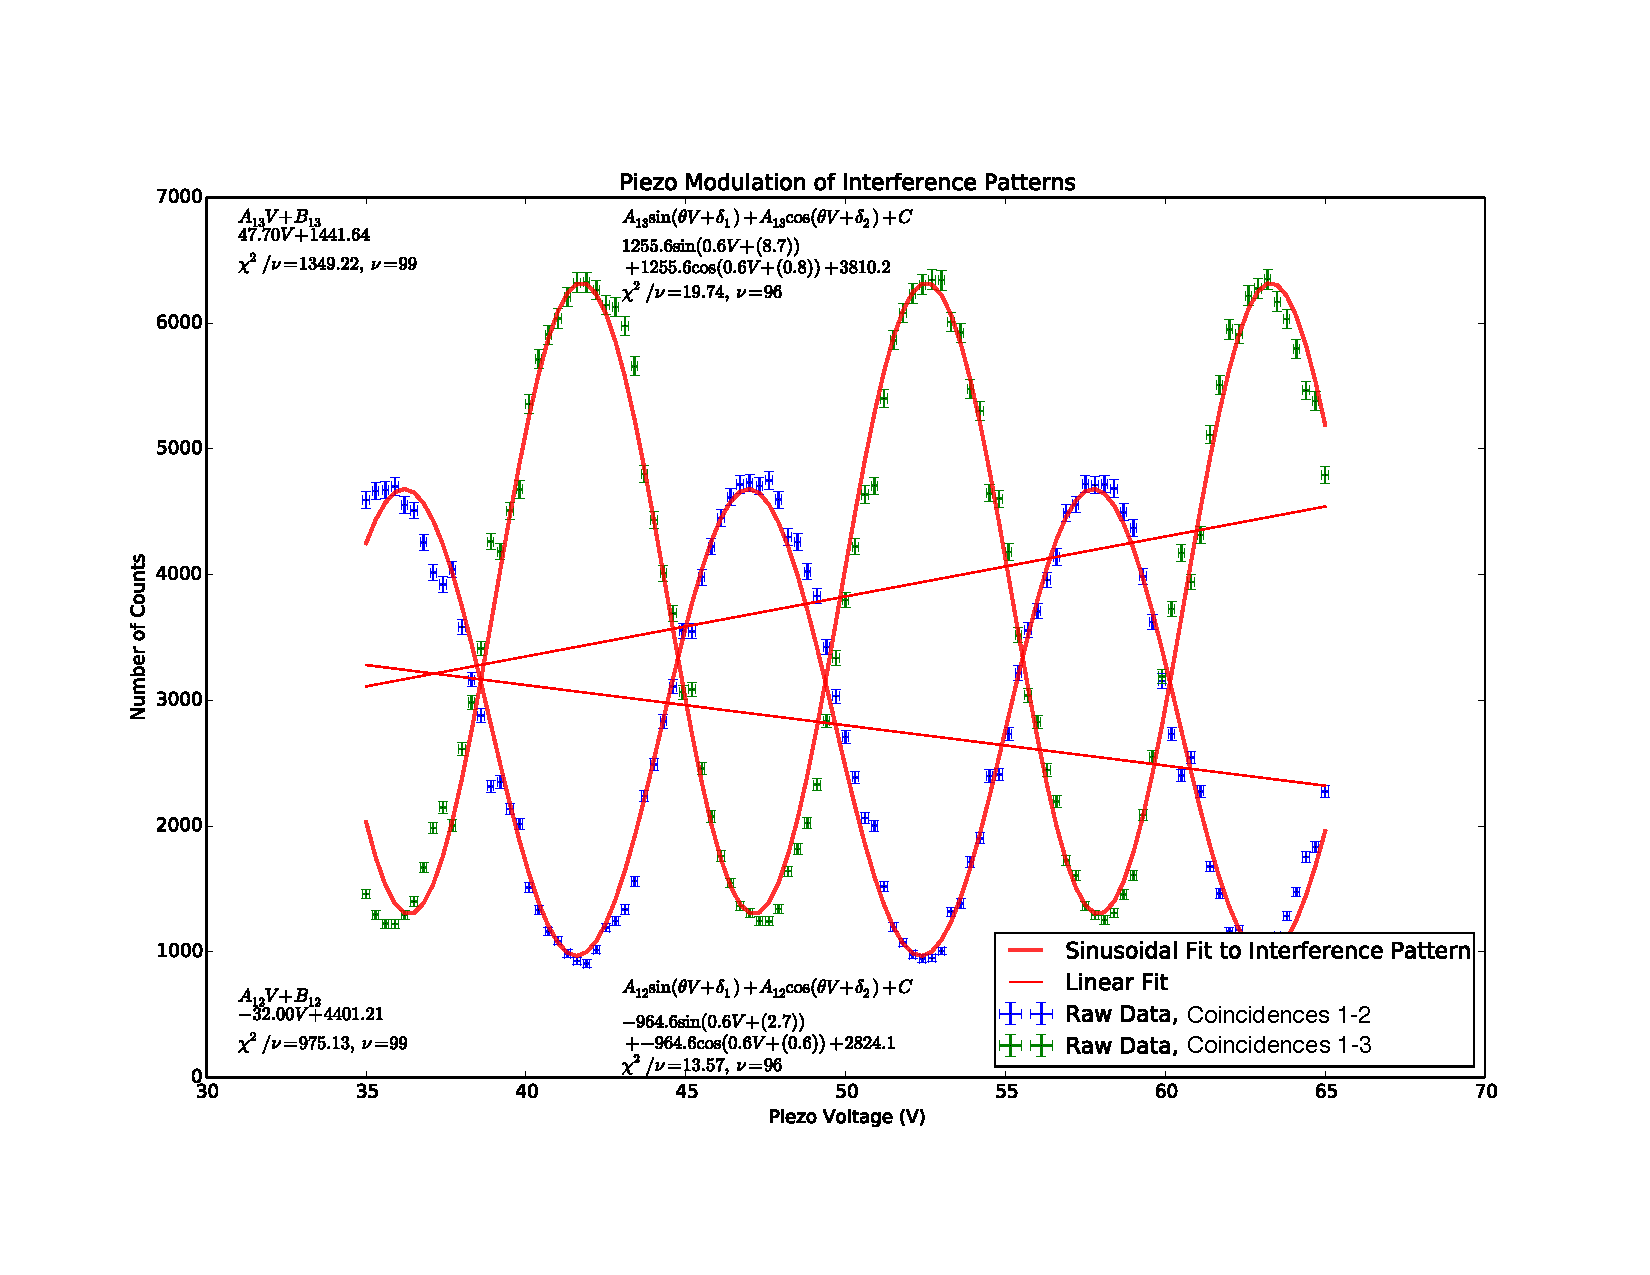
\includegraphics[scale=.525]{../plots/indistinguishable}
	\caption{The lines are clearly not good fits, and their \redchi values reflect this.  They are shown to give a sense of scale compared to the other plots.}
\end{figure}

\begin{table}[!htb]
	\centering
	\pgfplotstabletypeset[
   		precision=2,
   		every head row/.style={before row=\toprule, after row=\midrule},
   		every row no 4/.style={after row=\midrule},
   		every row no 9/.style={after row=\midrule},
   		every row no 11/.style={after row=\midrule},
   		every last row/.style={after row=\bottomrule},
   		columns/0/.style ={column type = {|c|},column name=Parameters},
   		columns/1/.style ={column type = {|c}, column name=Covariance Matrix},
   		columns/2/.style ={column type = {c}, column name=},
   		columns/3/.style ={column type = {c}, column name=},
   		columns/4/.style ={column type = {c}, column name=},
   		columns/5/.style ={column type = {c|}, column name=},
   		every even row/.style={before row={\rowcolor[gray]{0.9}}}]{../data/fitparms_indistinguishable.csv}
   		\caption{Zeroes indicate non-members of the covariance matrices, not a zero in that index.  This table is associated with the plot for the Indistinguishable Paths (Figure 4)}
\end{table}

Before we move on to actually performing some of the calculations detailed earlier on, we need to stop and discuss the massive error on our fit parameters.  This brief discussion will apply to all the subsequent fits as well.

\hspace{.25cm}

The first alarm should ring once the reader notices that our first parameter is $-372.62 \pm 6.54 \times 10^7$.  That is just incorrect, we essentially have no idea what the parameter is.  But the fit actually matches the data, with a low \redchi value.  This is where our knowledge of the covariance matrix will come in handy.  If we look at the covariance values, for example between A and $\delta_{1,2}$ we notice that element is $7.03 \times 10^5$.  That means that A and $\delta$ are \emph{highly} covariant.  Since the covariance matrix is related to the Jacobian of the system used to model the data and parameters we try to use to fit, we can imagine this as a complex landscape.  If we think about the covariance matrix as representative of that landscape, this simply tells us that the landscape slopes in more than one dimension, which should not be surprising, this is not a simple model.

\hspace{.25cm}

What we should therefore take away from this discussion is that we should place trust in the \redchi values in this case, as well as our own eyes.  In general, our eyes tell us that these fits are reliable, as does the \redchi value - letting us know that the covariant terms in the covariance matrix are causing problems.  We can estimate the variance of the parameters another way - by using something called the loss function, which is used by the fitting routine to actually perform the fit.  However, this is generally very complicated and the values of the loss function are not accessible if we run the scipy packages, so for now we must simply be content to know that the fits are acceptable.  Furthermore, we have nothing to compare to, and no literature values (that we know of) to compare to, so visual confirmation of the fit's efficacy is sufficient.

\hspace{.5cm}

Returning to the calculations described in the previous Theory section, we will calculate the approximate length of a photon.  Given that the downconverted photons have a wavelength of 810 nm ($\lambda$), and given that the bandwidth of the APD is approximately 10 nm ($\Delta \lambda$), we find that

\begin{gather}
	\Delta x \geq \frac{\lambda^2}{2\Delta \lambda} \\
	\Delta x \geq \frac{(810)^2}{20} nm \\
	\Delta x \geq 32,805 \, nm = 3.28 \times 10^{-5} \, m
\end{gather}

a value that is not terribly implausible.  One interesting feature of this value is that it will change based on how accurate our APD is, in terms of what we use for $\Delta \lambda$.  If we increase our sensitivity to wavelength (our bandwidth), we will see a photon that is longer, and vice-versa.  This seems counter-intuitive, but all it means is that there is an uncertainty relation between $x$ and $\lambda$.  In effect, we can say that

\begin{equation}
	\Delta x \Delta \lambda \geq \frac{1}{2} \lambda^2.
\end{equation}

If we treat the photon as a point particle, then $\Delta x$ is simply our uncertainty in its position, rephrased, its effective size.  Since the photon is anywhere within $\Delta x$, we realize that as our band decreases in size, we are more unsure of where the photon is, because we are more sure of its wavelength and vice-versa.

\hspace{.5cm}

Returning to the question of whether there will be more than one photon ever passing through the interferometer, we simply calculate the time in between counts, and realize that the spacing is such that only one photon ever passes through the interferometer.  We recorded the singles count rates with the laser on as approximately 100,000 ($\pm 8000$ for differences between APDs) in each APD (1,2,3 - I, A, B).

\begin{gather*}
	C.R. \approx 100,000 \, H\!z = 100,000 \, count/s \\
	c \, \sim \, \frac{[m]}{[s]} \\
	\implies c/C.R. \, \sim \, [m] \\
	D = c/C.R. \approx 3000 \, m 
\end{gather*}

This shows us that the distance between each photon is approximately 3000 m, far greater than any dimension of the optical table.

\begin{figure}[!htb]
	\centering
	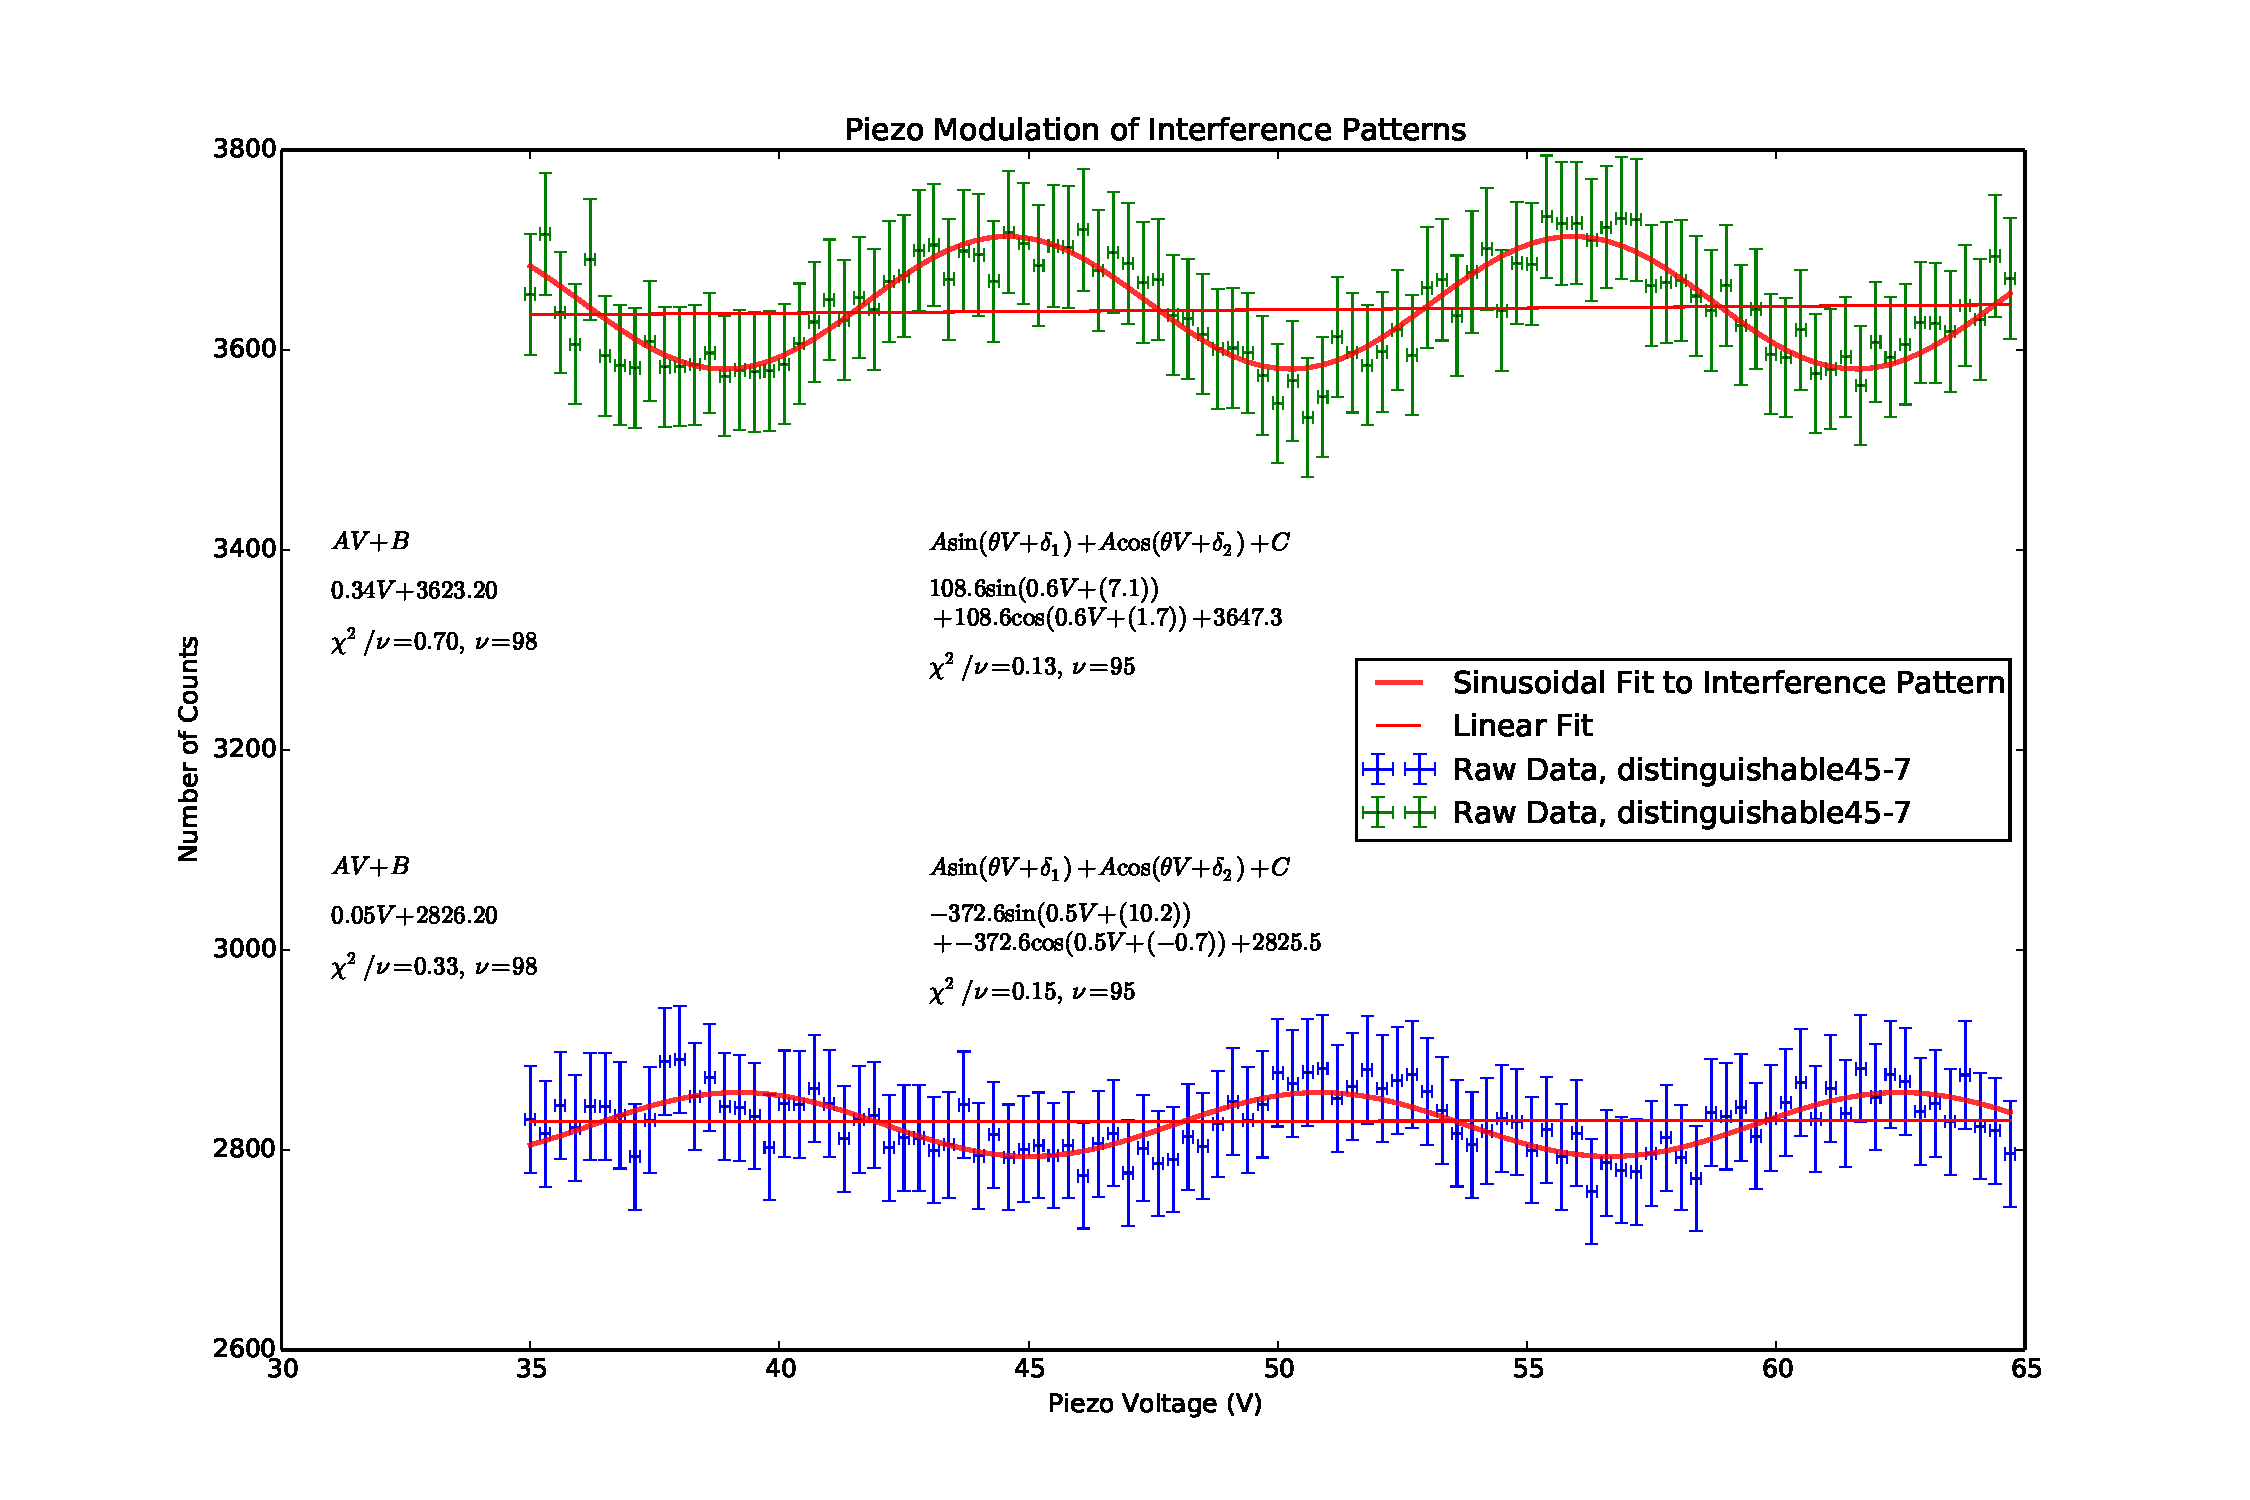
\includegraphics[scale=.525]{../plots/distinguishable45-7}
	\caption{The sin/cos models seem to fit well, however they overfit the data, as can be seen from their \redchi values of close to 0.  The lines fit the data quite well, as can be seen from their \redchi values of approximately 1.  Within uncertainties, the data stronly resemble a line, clearly.}
\end{figure}

\begin{table}[!htb]
	\centering
	\pgfplotstabletypeset[
   		precision=2,
   		every head row/.style={before row=\toprule, after row=\midrule},
   		every row no 4/.style={after row=\midrule},
   		every row no 9/.style={after row=\midrule},
   		every row no 11/.style={after row=\midrule},
   		every last row/.style={after row=\bottomrule},
   		columns/0/.style ={column type = {|c|},column name=Parameters},
   		columns/1/.style ={column type = {|c}, column name=Covariance Matrix},
   		columns/2/.style ={column type = {c}, column name=},
   		columns/3/.style ={column type = {c}, column name=},
   		columns/4/.style ={column type = {c}, column name=},
   		columns/5/.style ={column type = {c|}, column name=},
   		every even row/.style={before row={\rowcolor[gray]{0.9}}}]{../data/fitparms_distinguishable45-7.csv}
   		\caption{Zeroes indicate non-members of the covariance matrices, not a zero in that index.  This table is associated with the plot for the Distinguishable Paths (Figure 5)}
\end{table}

\begin{figure}[!htb]
	\centering
	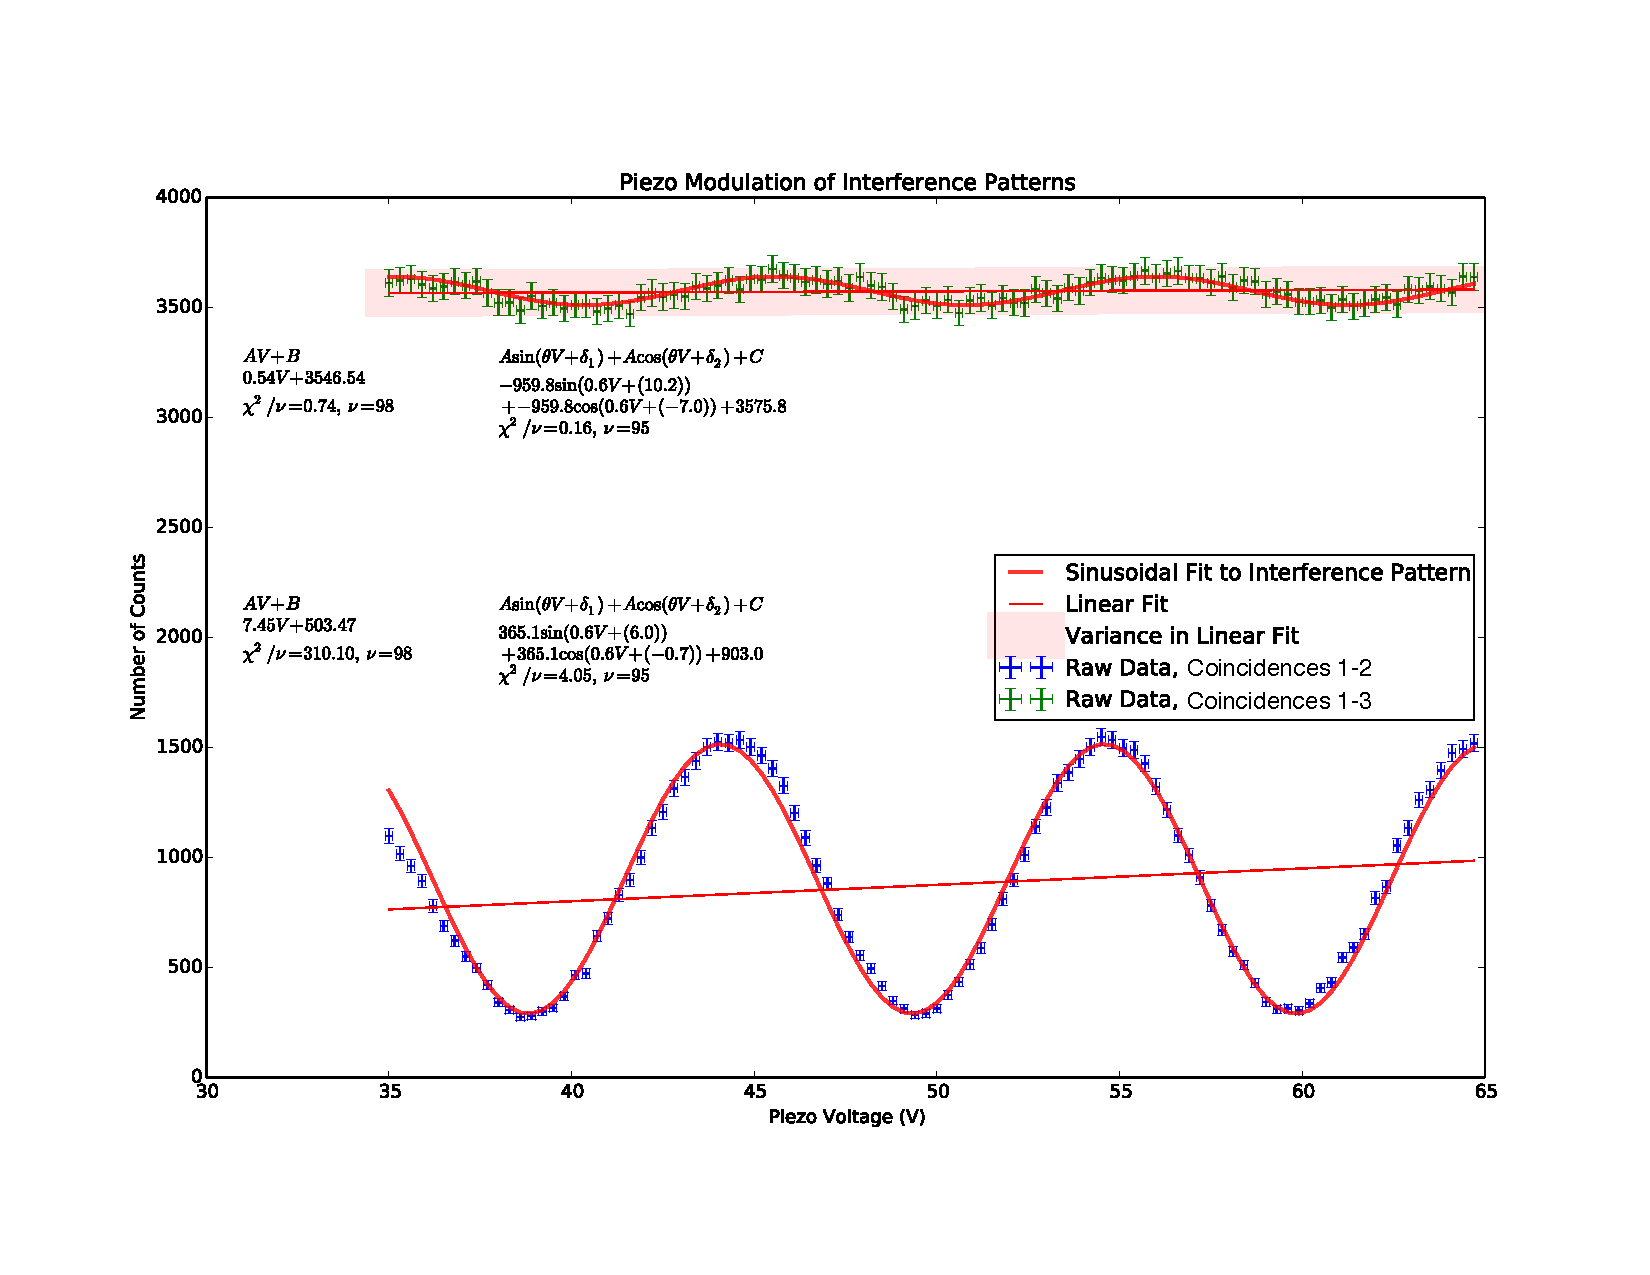
\includegraphics[scale=.525]{../plots/eraser}
	\caption{The red shaded region is the variance of the linear fit.  As we can see, it overlaps all the points and their uncertainties.}
\end{figure}

\begin{table}[!htb]
	\centering
	\pgfplotstabletypeset[
   		precision=2,
   		every head row/.style={before row=\toprule, after row=\midrule},
   		every row no 4/.style={after row=\midrule},
   		every row no 9/.style={after row=\midrule},
   		every row no 11/.style={after row=\midrule},
   		every last row/.style={after row=\bottomrule},
   		columns/0/.style ={column type = {|c|},column name=Parameters},
   		columns/1/.style ={column type = {|c}, column name=Covariance Matrix},
   		columns/2/.style ={column type = {c}, column name=},
   		columns/3/.style ={column type = {c}, column name=},
   		columns/4/.style ={column type = {c}, column name=},
   		columns/5/.style ={column type = {c|}, column name=},
   		every even row/.style={before row={\rowcolor[gray]{0.9}}}]{../data/fitparms_eraser.csv}
   		\caption{Zeroes indicate non-members of the covariance matrices, not a zero in that index.  The matrices are included because they play a significant role in these fits.  This table is associated with the Quantum Eraser plot (Figure 6)}
\end{table}

perform calculations that we talked about in the Theory section, equation numbers etc

\section{Conclusion}

\begin{thebibliography}{10}
	\bibitem{eff}
		Richard A. Myers, Richard Farrell, Arieh M. Karger, James E. Carey, and Eric Mazur, "Enhancing near-infrared avalanche photodiode performance by femtosecond laser microstructuring," Appl. Opt. 45, 8825-8831 (2006)

\end{thebibliography}

\end{document}